\chapter{Quanten-Teleportation\label{chapter:teleport}}
\lhead{Quanten-Teleportation}
\begin{refsection}
\chapterauthor{Max Obrist und Martin Stypinski}

\section{Einleitung}

Die Quantenteleportation beschreibt die M"oglichkeit, Quantenzust"ande "uber eine Distanz zu transportieren. Die Kernidee bei der Quantenteleportation ist nicht die "Ubertragung von Quanten, sondern viel mehr die "Ubertragung der Information. Ein Quantenzustand soll quasi von A nach B transportiert werden. Die Information soll "uber einen 'Informationskanal' "ubertragen werden, die Quanten an sich aber werden im eigentlichen Sinne nicht "ubertragen, da sie sehr leicht ihren Zustand "andern. Die Quantenteleportation ist somit ein Verfahren zur Kommunikation zwischen mehreren Teilnehmern.

Als Quellen dieser Erl"auterungen wurden eine Masterarbeit \cite{teleport:mscthesis} und ein Seminarvortrag \cite{teleport:teleport-seminar} verwendet.

\section{Problem}
\rhead{Problem}
\subsection{Klassische Kommunikation}
Angefangen bei der klassischen Kommunikation, kann man die Informations"ubertragung sehr einfach darstellen. Der Sender Alice verpackt seine Information in eine Kiste. Diese wird mittels einem Speditionsunternehmen zu Bob transportiert. Bob "offnet die Kiste und findet die Information wieder. Die Kommunikation zwischen Alice und Bob konnte somit stattfinden. Dies ist sehr einfach und anschaulich erkl"art und ben"otigt eine 'physische' "Ubertragung der Information. Einfacher ist es mit einem Faxger"at: Der Sender Alice faxt seine Meldung zu Empf"anger Bob. In der Informatik selbst w"are es die "Ubertragung von Bits. Alice und Bob haben somit Informationen ausgetauscht.
\begin{figure}
\center
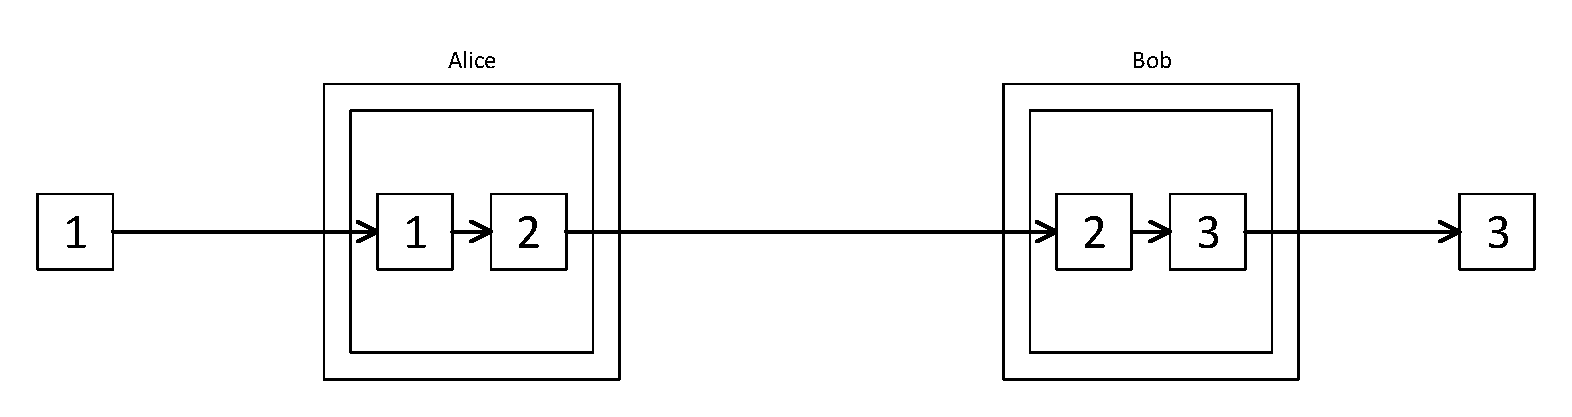
\includegraphics[width=1\textwidth]{teleport/image/classic_com.pdf}
\caption{Klassische Kommunikation von Alice zu Bob.}
\label{Klassische Kommunikation}
\end{figure}
\subsection{Quantenmechanisches Problem}
Das Problem in der Quanteninformatik ist, dass der Zustand eines Teilchens nicht ohne Weiteres von Alice zu Bob "ubertragen werden kann. Besitzt Alice ein Teilchen im Zustand $\left|\phi\right\rangle$, kann sie dessen Zustand nicht ohne weiteres an Bob "ubertragen. Der naive Versuch einfach das Teilchen zu "ubertragen, birgt verschiedene technische Schwierigkeiten mit sich. Es ist "ausserst schwierig, ein Teilchen unver"andert "uber gr"ossere Distanzen zu transportieren. F"ur den gesamten Transportweg m"ussten s"amtliche Wechselwirkungen eliminiert werden. 

Die Heisenbergschen Unsch"arferelation zeigt ausserdem, dass es Alice unm"oglich ist, das zu "ubertragende Teilchen so zu messen, dass Bob daraus den Originalzustand rekonstruieren k"onnte (Reduktionspostulat). Nehmen wir zur Illustration die Polarisationsrichtung eines Photons. Das Photon befindet sich in einem Zustand $\left|\phi\right\rangle$, welcher eine Superposition aus den Zust"anden $\left|\leftrightarrow\right\rangle$ (horizontal polarisiert) und $\left|\updownarrow\right\rangle$ (vertikal polarisiert) darstellt. Das System $\left|\phi\right\rangle$ l"asst sich somit formal schreiben als
\begin{align}\label{eq:qubit1}
\left|\phi\right\rangle = \alpha\left|\leftrightarrow\right\rangle + \beta\left|\updownarrow\right\rangle 
\end{align}
mit $\alpha, \beta \in \mathbb{C}$ und der Bedingung $\left|\alpha\right|^{2} + \left|\beta\right|^{2} = 1$. Im Folgenden verwenden wir die "ublichere Notation f"ur 2-Zustandsysteme und schreiben die beiden Zust"ande als $\left| 0 \right\rangle$ (horizontal polarisiert) und $\left| 1 \right\rangle$ (vertikal polarisiert). Das auch unter dem Namen Qubit bekannte System l"asst sich dann schreiben als 
\begin{align}\label{eq:qubit2}
\left|\phi\right\rangle = \alpha\left|0\right\rangle + \beta\left|1\right\rangle.
\end{align}

Misst man nun ein System, welches mit Gleichung (\ref{eq:qubit1}) beschrieben wird, hat eine Messung der Spinkomponente folgende Wahrscheinlichkeiten:
\begin{align}
	\begin{split}
		P\left(\leftrightarrow\right) & =\left|\alpha\right|^2  \\
	    P\left(\updownarrow\right) & =\left|\beta\right|^2
	\end{split}
\end{align}

F"uhrt man eine Messung von $\left|\phi\right\rangle$ durch und bestimmt damit entweder $\alpha$ oder $\beta$, wird die Superposition des Teilchens zerst"ort und es befindet sich in einem der Basiszust"ande $\left|\leftrightarrow\right\rangle$ oder $\left|\updownarrow\right\rangle$. Die jeweils andere Komponente l"asst sich nun nicht mehr bestimmen. Es scheint also unm"oglich, den vollst"andigen Zustand eines Teilchens mit einer Messung zu bestimmen.

\section{Quantenteleportationsprozess}
\rhead{Quantenteleportationsprozess}
\index{Quantenteleportationsprozess}%
Auch wenn die Heisenbergsche Unsch"arferelation dem Vorhaben von Alice, ein Teilchen zu Bob zu schicken, auf den ersten Blick im Wege steht, ist es genau dasselbe Prinzip, welche bei der Quantenteleportation -- zusammen mit der Quantenverschr"ankung -- eine zentrale Rolle spielt.
\begin{figure}
	\center
	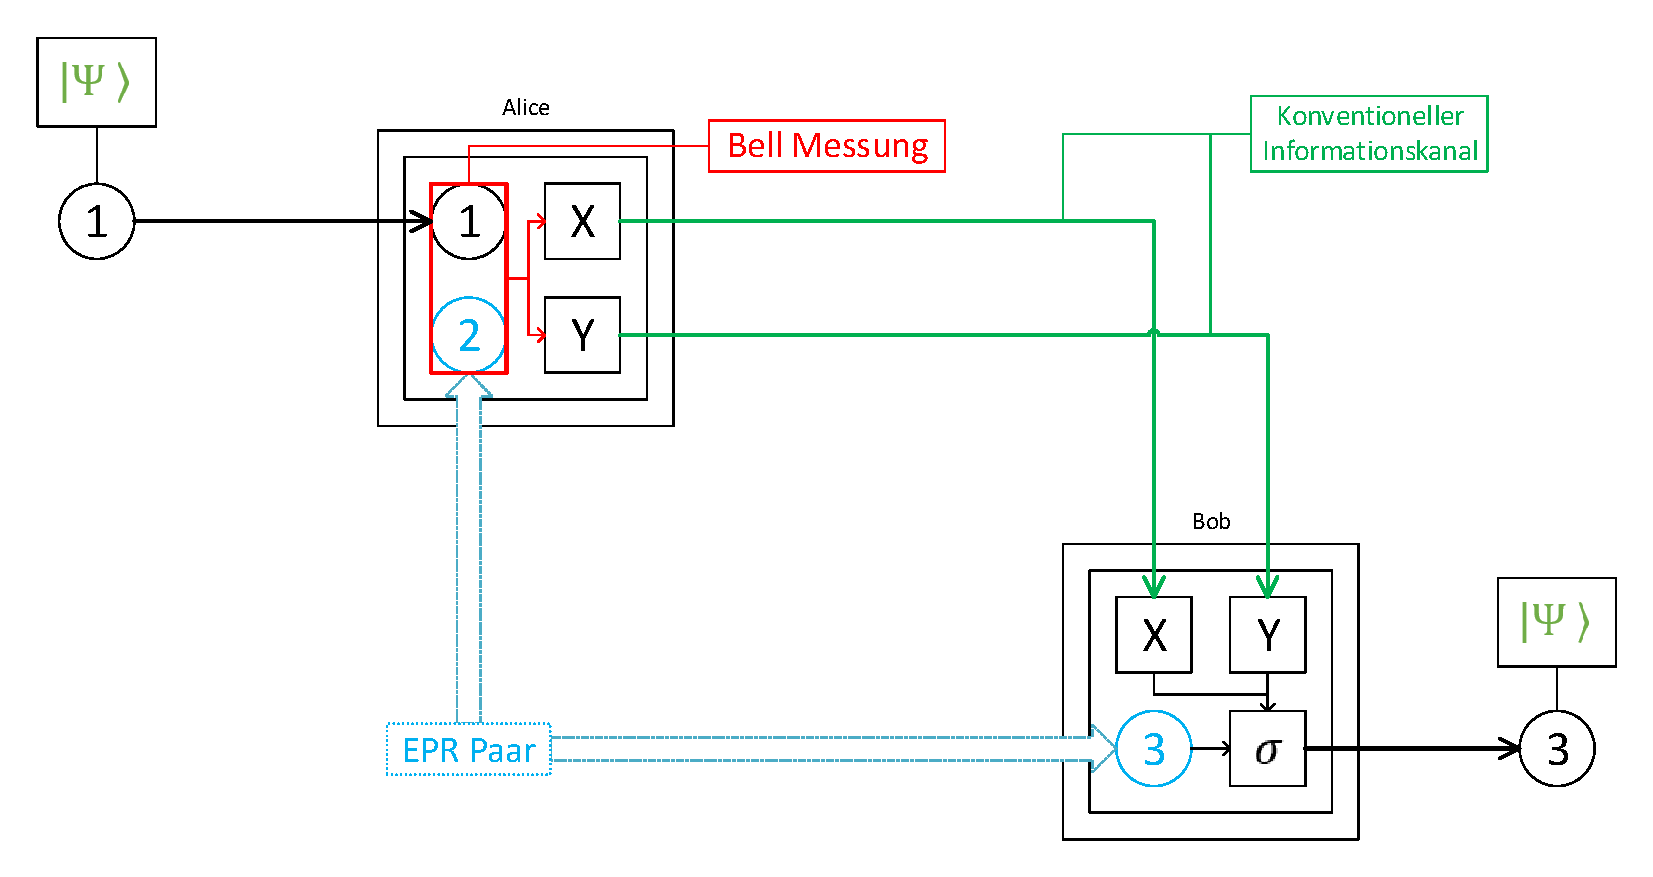
\includegraphics[width=1\textwidth]{teleport/image/quantum_com.pdf}
	\caption{Quantenteleportation}
	\label{Quantenteleportation}
\end{figure}

\subsection{Voraussetzungen}

Voraussetzung f"ur den Quantenteleportationsprozess ist, dass Alice und Bob je ein Teilchen eines verschr"ankten Paares besitzen, die Teilchen $T_{2}$ und $T_{3}$. Da die beiden Teilchen  verschr"ankt sind, lassen sie sich nur gemeinsam beschreiben, der Zustand der einzelnen Teilchen l"asst sich allerdings nicht bestimmen. Die beiden Teilchen k"onnen sich in einem von vier verschr"ankten Paarzust"anden befinden, den sogenannten Bell States. Im Abschnitt~\ref{sec:bell-states} werden diese noch genauer angeschaut und sind f"ur das Verst"andnis des Quantentelportationsprozesses vorerst noch nicht relevant. Man behalte sich allerdings im Hinterkopf, dass sich alle verschr"ankten Paare w"ahrend dem Prozess in einem Bellschen Zustand befinden.

Ein solches verschr"anktes Paar in einem Bell State nennt sich auch EPR-Paar. F"ur unser Beispiel nehmen wir an, dass sich das Paar in folgendem Zustand befindet:
\index{EPR-Paar}%
\begin{align}\label{eq:bell_state1}
\left|\Psi^{-}\right\rangle_{23} = \frac{1}{\sqrt{2}} ( \left|0\right\rangle_{2}\left|1\right\rangle_{3} - \left|1\right\rangle_{2}\left|0\right\rangle_{3} )
\end{align}

Dieser Zustand erlaubt keinerlei R"uckschl"usse auf den eigentlichen Zustand von $T_{2}$ und $T_{3}$. Er sagt einzig aus, dass sich $T_{2}$ und $T_{3}$ in orthogonalen Zust"anden befinden. Aus einer Messung von $T_{2}$ l"asst sich der Zustand von $T_{3}$ bestimmen, zerst"ort aber gleichzeitig den Zustand von $T_{2}$. 

\subsection{Teleportationsvorgang}\label{sec:teleportation}

Nun erh"alt Alice ein Teilchen $T_{1}$ im unbekannten Zustand $\left|\phi\right\rangle = \alpha\left|0\right\rangle + \beta\left|1\right\rangle$. Sie f"uhrt nun eine sogenannte Bellsche Zustandsmessung auf $T_{1}$ und $T_{2}$ durch.

Wir betrachten im Abschnitt~\ref{sec:bell-measurement} genauer, was bei dieser Messung geschieht. F"ur diese Erl"auterung ist wichtig, was bei der Bell-Messung am Ende herauskommt. Das Ergebnis der Bell-Messung sagt uns, in welchem der vier Bell States sich die beiden Teilchen befinden. Befinden sich die Teilchen nicht bereits in einem solchen Zustand, werden sie auf einen Bellschen Zustand projiziert. Da alle Bell States verschr"ankt sind, ist die Bell-Messung auch eine verschr"ankende Operation.

Die Teilchen $T_{1}$ und $T_{2}$ sind also neu miteinander verschr"ankt, was bedeutet, dass $T_{1}$ seinen Identit"at verliert und nur noch gemeinsam mit $T_{2}$ beschreibbar ist. Der Zustand von $T_{1}$ und $T_{2}$ l"asst sich genau mit dem in der Messung erhaltenen Bell State beschreiben. 

Gleichzeitig sind auch die Teilchen $T_{2}$ und $T_{3}$ noch miteinander verschr"ankt, und zwar im Zustand (\ref{eq:bell_state1}). Wie erw"ahnt handelt es sich auch bei dieser Gleichung um einen Bellschen Zustand.

Nehmen wir nun an, die Bellsche Zustandsmessung bei Alice hat als Ergebnis den folgenden Zustand:
\begin{align}\label{eq:bell_state2}
\left|\Psi^{-}\right\rangle_{12} = \frac{1}{\sqrt{2}} ( \left|0\right\rangle_{1}\left|1\right\rangle_{2} - \left|1\right\rangle_{1}\left|0\right\rangle_{3} )
\end{align}
Die Teilchen $T_{1}$ und $T_{2}$ befinden sich somit im selben Bell State $\left| \Psi^{-} \right \rangle$ wie $T_{2}$ und $T_{3}$ und sind damit ebenfalls orthogonal zueinander. Nun existiert folgende Situation: $T_{1}$ und $T_{2}$ sind miteinander verschr"ankt und befinden sich im Zustand~(\ref{eq:bell_state2}), sind also orthogonal ausgerichtet. $T_{2}$ und $T_{3}$ sind ebenfalls miteinander verschr"ankt und befinden sich im selben Zustand~(\ref{eq:bell_state1}), sind also ebenfalls verschr"ankt und stehen orthogonal zueinander. Dies bedeutet, dass sich die Teilchen $T_{1}$ und $T_{3}$ -- abgesehen von einem unwichtigen Phasenvektor -- im selben Zustand befinden m"ussen: $\left| \Psi\right\rangle_{3} = -\left|\phi\right\rangle$.

\subsection{Bellsche Zust"ande}\label{sec:bell-states}
\index{Bellsche Zustande@Bellsche Zust\"ande}%

% XXX bei "wird dabei einerseits" verunglückt der Satz
Im Abschnitt~\ref{sec:teleportation} wurde das grunds"atzliche Konzept der Quantenteleportation erl"autert. Dabei wurde allerdings die Bellsche Zustandsmessung bewusst weggelassen. Diese ist "ausserst zentral bei der Quantenteleportation, wird dabei einerseits das zu teleportierende Teilchen $T_{1}$ mit $T_{2}$ verschr"ankt, welches Teil des Bell Paares ist, das sich Alice und Bob teilen. Andererseits ergibt sie als Resultat auch den Bellschen Zustand, in welchem sich die Teilchen $T_{1}$ und $T_{2}$ befinden. Dies erlaubt es Bob "uberhaupt, den urspr"unglichen Zustand in $T_{3}$ wiederherzustellen. Die Bellsche Zustandsmessung stellt sich bei der experimentellen Realisierbarkeit als "ausserst Komplex heraus und ist eines der Hauptprobleme der Quantenteleporation. Darauf wird in diesem Rahmen aber nicht eingegangen.

Das Resultat der Bell Messung ist einer der vier Bell States. Diese vier Bell States sind sogenannt maximal verschr"ankte Zust"ande. Die einzelnen Bell States sehen folgendermassen aus:
\begin{align}
	\begin{split}
\left|\Phi^+\right\rangle & = \frac{1}{\sqrt{2}}(\left|0\right\rangle_{A}\left|0\right\rangle_{B} + \left|1\right\rangle_{A}\left|1\right\rangle_{B}) \\
\left|\Phi^-\right\rangle & = \frac{1}{\sqrt{2}}(\left|0\right\rangle_{A}\left|0\right\rangle_{B} - \left|1\right\rangle_{A}\left|1\right\rangle_{B}) \\
\left|\Psi^+\right\rangle & = \frac{1}{\sqrt{2}}(\left|0\right\rangle_{A}\left|1\right\rangle_{B} + \left|1\right\rangle_{A}\left|0\right\rangle_{B}) \\
\left|\Psi^-\right\rangle & = \frac{1}{\sqrt{2}}(\left|0\right\rangle_{A}\left|1\right\rangle_{B} - \left|1\right\rangle_{A}\left|0\right\rangle_{B}) 
	\end{split}
\end{align}

\subsection{Bellsche Zustandsmessung}\label{sec:bell-measurement}
\index{Bell Messung}%

Nachdem wir die 4 Bellschen Zust"ande betrachten haben, gehen wir nun zur eigentlichen Zustandsmessung "uber. Betrachten wir daf"ur erneut das Bell Paar, welches sich Alice und Bob vor dem Teleportationsvorgang teilen:
\begin{align}  \tag{\ref{eq:bell_state1}}
 \left|\Psi^{-}\right\rangle_{23} = \frac{1}{\sqrt{2}} ( \left|0\right\rangle_{2}\left|1\right\rangle_{3} - \left|1\right\rangle_{2}\left|0\right\rangle_{3} ).
\end{align}

Erh"alt Alice nun das zu teleportierende Teilchen $T_{1}$ im Zustand $\left|\phi\right\rangle = \alpha\left|0\right\rangle + \beta\left|1\right\rangle_{1}$ ergibt sich ein Gesamtsystem aus 3 Teilchen
\begin{align}\label{eq:full_system1}
\left|\Psi_{123}\right\rangle = \left| \phi, \Psi^{-} \right\rangle = \big( \alpha \left| 0 \right\rangle + \beta \left| 1 \right\rangle \big) \otimes \big( \frac{1}{\sqrt{2}} ( \left|0\right\rangle \left|1\right\rangle - \left|1\right\rangle \left|0\right\rangle ) \big)
\end{align}
Durch Ausmultiplizieren und Zusammenfassen ergibt sich daraus:
\begin{align}\label{eq:full_system2}
\left|\Psi_{123}\right\rangle = \frac{\alpha}{\sqrt{2}} \big(\left|0, 0, 1 \right\rangle - \left|0, 1, 0 \right\rangle  \big) + \frac{\beta}{\sqrt{2}} \big(\left|1, 0, 1 \right\rangle - \left|1, 1, 0 \right\rangle \big)
\end{align}

Ein Trick des Ganzen ist die Darstellung dieses Zustandes in einer anderen Basis. Der Hilbertraum, in welchem (\ref{eq:full_system2}) dargestellt ist, hat als Basis die 8 Produktzust"ande
\begin{align}
\left|  0,0,0 \right \rangle,\left|  0,0,1 \right \rangle,\left|  0,1,0 \right \rangle,\left|  0,1,1 \right \rangle,\left|  1,0,0 \right \rangle,\left|  1,0,1 \right \rangle,\left|  1,1,0 \right \rangle,\left|  1,1,1 \right \rangle.
\end{align}

Mathematisch betrachtet ist es allerdings m"oglich, eine andere Basis f"ur den Hilbertraum zu w"ahlen. Nimmt man als Basis die Produktzust"ande der vier Bell States ($\left|\Phi^+\right\rangle$, $\left|\Phi^-\right\rangle$, $\left|\Psi^+\right\rangle$, $\left|\Psi^-\right\rangle$, das verschr"ankte EPR-Paar von Alice und Bob) mit den beiden Zust"anden eines einzelnen Qubits ($\left|0\right\rangle$ und $\left|1\right\rangle$, das zu teleportierende Teilchen $T_{1}$) erh"alt man folgende Basis f"ur den Hilbertraum:
\begin{align}
\left|\Phi^{+}_{12},0\right\rangle,
\left|\Phi^{+}_{12},1\right\rangle, 
\left|\Phi^{-}_{12},0\right\rangle,
\left|\Phi^{-}_{12},1\right\rangle,
\left|\Psi^{+}_{12},0\right\rangle,
\left|\Psi^{+}_{12},1\right\rangle,
\left|\Psi^{-}_{12},0\right\rangle,
\left|\Psi^{-}_{12},1\right\rangle.
\end{align}

Stellt man nun den Zustand~(~\ref{eq:full_system2}~) in dieser Basis dar, erh"alt dieser die Form
\begin{align}\label{eq:full_system3}
	\begin{split}
\left| \Psi_{123} \right\rangle = \frac{1}{2} \Bigg( \left| \Psi_{12}^{+} \right\rangle (-\alpha \left| 0 \right\rangle + \beta \left| 1 \right\rangle) - \left| \Psi_{12}^{-} \right\rangle (\alpha \left| 0 \right\rangle + \beta \left| 1 \right\rangle ) +
\\
+ \left| \Phi_{12}^{+} \right\rangle (\alpha \left| 1 \right\rangle - \beta \left| 0 \right\rangle) + \left| \Phi_{12}^{-} \right\rangle (\alpha \left| 1 \right\rangle + \beta \left| 0 \right\rangle
 \Bigg).
 \end{split}
\end{align}
Auf die Umrechnung soll hier verzichtet werden.

Nun kommt der zweite Trick; die eigentliche Bellsche Zustandsmessung. Alice f"uhrt eine solche auf ihren beiden Teilchen aus. Sie stellt also fest, in welchem Bell Zustand sie sich befinden, oder projiziert sie auf einen solchen. Wie bei jeder Messung wird das Gesamtsystem (\ref{eq:full_system3}) auf einen anderen Zustand projiziert -- es reduziert sich auf einen einzelnen Summanden. Der "ubrig bleibende Summand h"angt davon ab, in welchem Bell Zustand sich $T_{2}$ und $T_{3}$ befinden und auf welchen Zustand $T_{1}$ und $T_{2}$ projiziert wurden. In unserem Beispiel nahmen wir an, das sich beide System im Zustand $\left|\Psi_{12}^{-}\right\rangle$ befanden. In diesem Fall kollabriert das Gesamtsystem zu
\begin{align}
\left| \Psi_{123}^{(1)} \right\rangle = \frac{1}{2} \left| \Psi_{12}^{-} \right \rangle (-\alpha \left| 0 \right \rangle - \beta \left| 1 \right\rangle).
\end{align}

$T_{3}$ befindet sich somit in einem Zustand, welcher bis auf einen konstanten Vorfaktor $-\frac{1}{2}$ dem von $T_{1}$ im Originalzustand entspricht:
\begin{align}
\left| \psi_{3}^{(1)} \right\rangle = - \frac{1}{2} \left( \alpha \left| 0 \right \rangle + \beta \left| 1 \right \rangle \right ) = - \frac{1}{2} \left| \phi \right \rangle
\end{align}
F"ur die weitere Verwendung ist dieser Vorfaktor irrelevant. Die Teleporation des Zustandes war somit erfolgreich. 

Bisher haben wir  nur betrachtet, was geschieht, wenn Alice bei der durchgef"uhrten Bell Messung denselben Bell Zustand erh"alt, in dem sich auch das EPR-Paar von Alice und Bob befand. Dies geschieht aber nur mit einer Wahrscheinlichkeit von $\frac{1}{4}$. Mit einer Wahrscheinlichkeit von $\frac{3}{4}$ misst Alice also einen der anderen 3 m"oglichen Zust"ande. F"ur den Abschluss des Teleportationsvorganges ist in diesem Fall noch ein weiterer Schritt n"otig.

F"ur jedes Messergebnis von Alice ist aber jeweils bekannt, in welchem Zustand sich Bobs Teilchen befinden muss. In der folgenden Tabelle wurde der physikalisch gesehen unwichtige Faktor $-\frac{1}{2}$ weggelassen.
\begin{center}
   \begin{tabular}{| l | l |}
   \hline
   Alices Zustand & Zustand von Bobs Teilchen \strut \\
    \hline
     \raisebox{0mm}[5mm][3mm]{}$\left| \Psi_{12}^{-} \right\rangle$ & $ \left| \psi_{3}^{(1)} \right\rangle := \alpha \left| 0 \right \rangle + \beta \left| 1 \right \rangle $ \\ \hline
     \raisebox{0mm}[5mm][3mm]{}$\left| \Psi_{12}^{+} \right\rangle$ & $ \left| \psi_{3}^{(2)} \right\rangle := -\alpha \left| 0 \right \rangle + \beta \left| 1 \right \rangle $ \\ \hline
     \raisebox{0mm}[5mm][3mm]{}$\left| \Phi_{12}^{-} \right\rangle$ & $ \left| \psi_{3}^{(3)} \right\rangle := \beta \left| 0 \right \rangle + \alpha \left| 1 \right \rangle $ \\ \hline
     \raisebox{0mm}[5mm][3mm]{}$\left| \Phi_{12}^{+} \right\rangle$ & $ \left| \psi_{3}^{(4)} \right\rangle := -\beta \left| 0 \right \rangle + \alpha \left| 1 \right \rangle $ \\ \hline
   \end{tabular}
\end{center}

Auffallend ist, dass $\left| \psi_{3}^{(i)} \right\rangle$ zwar jeweils dieselben Koeffizienten wie $\left| \phi \right\rangle$ besitzen, diese aber z.T. vertauscht sind oder unterschiedliche Vorzeichen besitzen. Dies bedeutet, dass die drei Zust"ande kein skalares Vielfaches von $\left| \phi \right\rangle$ sind.

Damit Bob sein Teilchen in den richtigen Zustand "uberf"uhren kann, muss er nur noch eine einfache unit"are Transformation auf seinem Teilchen $T_{3}$ durchf"uhren. Die geltenden Zusammenh"ange werden hier aufgelistet. Der Vollst"andigkeit halber ist auch die Matrix im Falle von $\left|\phi_{3}^{(1)}\right\rangle$ nochmals aufgelistet.
\begin{align}
	\left| \psi_{3}^{(1)} \right \rangle & = \begin{pmatrix} 1 & 0 \\ 0 & 1 \end{pmatrix} \left| \phi \right \rangle \\
	\left| \psi_{3}^{(2)} \right \rangle & = \begin{pmatrix} -1 & 0 \\ 0 & 1 \end{pmatrix} \left| \phi \right \rangle \\
	\left| \psi_{3}^{(3)} \right \rangle & = \begin{pmatrix} 0 & 1 \\ 1 & 0 \end{pmatrix} \left| \phi \right \rangle \\
	\left| \psi_{3}^{(4)} \right \rangle & = \begin{pmatrix} 0 & -1 \\ 1 & 0 \end{pmatrix} \left| \phi \right \rangle
\end{align}

Damit Bob die richtige unit"are Matrix ausw"ahlen kann, muss ihm Alice somit zuerst das Resultat der Bellschen Zustandsmessung mitteilen. Bob hat ohne dieser Information keine M"oglichkeit, die richtige Matrix mit einer besseren Wahrscheinlichkeit als $\frac{1}{4}$ auszuw"ahlen. Deshalb ist die konventionelle "Ubertragung des Messergebnisses zu Bob n"otig. Dies erkl"art auch, warum die  Quantenteleportation keine "uberlichtschnelle Kommunikation erlaubt und somit die Gesetze der Relativit"atstheorie nicht verletzt werden.

Es ist noch darauf hinzuweisen, dass sich in dieser Erl"auterung das EPR-Paar von Alice und Bob, die Teilchen $T_{2}$ und $T_{3}$, im Zustand $\left| \Phi^{-} \right\rangle$ befanden. Dies ist keine Einschr"ankung des Protokolls, sondern diente der einfacheren Erl"auterung. Das EPR-Paar kann sich in jedem beliebigen der 4 Bell Zust"ande befinden. Gleichungen (\ref{eq:full_system1}), (\ref{eq:full_system2}) und (\ref{eq:full_system3}) w"urden in diesem Fall etwas anders aussehen, h"atten aber dieselbe Grundstruktur.

\section{Schlussfolgerung}
\rhead{Schlussfolgerung}

Nach dem Vorgang der Quantenteleportation wurde also der Zustand des Teilchens $T_{1}$ auf das Teilchen $T_{3}$ projiziert. Dabei wurde der Zustand von $T_{1}$ zerst"ort, das No-Cloning Theorem wird also nicht verletzt. Bemerkenswert an dem Vorgang ist auch, dass weder Alice noch Bob zu irgendeinem Zeitpunkt Informationen "uber die Zust"ande der einzelnen Teilchen $T_{1}$, $T_{2}$ und $T_{3}$ hatten, insbesondere nicht "uber den zu teleportierenden Zustand $\left|\phi\right\rangle$. 

Interessant ist auch, dass auf diese Weise auch verschr"ankte Systeme "ubertragen werden k"onnen. Haben wir ein System von zwei verschr"ankten Teilchen $T_{X}$ und $T_{Y}$, und wird $T_{X}$ zu Bob teleportiert, sind $T_{Y}$ bei Alice und $T_{X}$ bei Bob weiterhin verschr"ankt. Wird nun auch $T_{Y}$ zu Bob teleportiert, sind $T_{X}$ und $T_{Y}$ nat"urlich ebenfalls weiterhin miteinander verschr"ankt. Dieser Vorgang l"asst sich auf beliebig komplexe verschr"ankte Systeme erweitern. 

Somit haben wir einen Weg gefunden, wie wir den Zustand eines Teilchens -- und damit seine Information -- zu einem beliebigen Ziel senden k"onnen, ohne die Gesetze der Quantenmechanik zu verletzen, und ohne extrem aufwendige Massnahmen treffen zu m"ussen, um Wechselwirkungen mit der Umgebung zu vermeiden. Der dem Vorgang zugrundeliegende Effekt der Quantenverschr"ankung konnte "ubrigens schon "uber eine Distanz von bis zu 143 Kilometer nachgewiesen, und zwar zwischen den beiden kanarischen Inseln La Palma und Teneriffa.
\index{La Palma}
\index{Teneriffa}
\section{Anwendung}

Auch wenn es durch die Quantenteleportation leider nicht m"oglich sein wird, Gegenst"ande oder gar Personen zu teleportieren, gibt es trotzdem verschiedene interessante Anwendungsgebiete

\subsection{Quantencomputer}

In einem Quantencomputer ist die "Ubertragung der Zust"ande zwischen einzelnen Komponenten von zentraler Bedeutung. Dies k"onnte mittels der Quantenteleportation realisiert werden.

\subsection{Quantenkryptographie} 
Das No-Cloning Theorem besagt, dass der Zustand eines Teilchens nicht kopiert werden kann. Die Heisenbergsche Unsch"arferelation sagt aus, dass es unm"oglich ist, den vollst"andigen Zustand eines Teilchens auszumessen. Sobald eine Messung erfolgt, beeinflusst diese die Quantenzust"ande und die Information, die "ubertragen werden soll, ist somit ver"andert. Dies garantiert, dass ein potentieller Mith"orer immer erkannt werden kann. N"aheres dazu im Abschnitt zur Kryptographie. \ref{chapter:crypto}

\printbibliography[heading=subbibliography]
\end{refsection}
